\documentclass[11pt,a4paper]{article}

\usepackage[utf8]{inputenc}
\usepackage[T1]{fontenc}
\usepackage[turkish,shorthands=:!]{babel}   % '=' kisaltmasini kapat (tikz/enumitem ile cakisiyor)
\usepackage{lmodern}
\usepackage[margin=2.3cm]{geometry}
\usepackage{amsmath,amssymb}
\usepackage{booktabs}
\usepackage{xcolor}
\usepackage{listings}
\usepackage{graphicx}
\usepackage{float}
\usepackage{tikz}
\usetikzlibrary{arrows.meta,positioning,babel}
\usepackage[american]{circuitikz}
\usepackage{enumitem}
\usepackage{parskip}
\usepackage{url}

\lstset{basicstyle=\ttfamily\small, columns=fullflexible, frame=single,
        framesep=4pt, rulecolor=\color{black!30}, backgroundcolor=\color{black!3}}


\title{DC Motorlu Tek Eklemli Robot Kolu\\[2pt] \large Durum Uzayı Modeli ve Açık Çevrim Simülasyonu}
\author{Şafak Şahin}
\date{EEM5507 Doğrusal Sistemler Teorisi, 2026--27 Güz}

\begin{document}
\maketitle

\noindent\textit{Not: Bu belge EEM5507 Ödev 1'in KT1 (proje başlangıcı) bölümüdür. Metindeki ``Soru 2'', ``Soru 4'' atıfları ödevin diğer sorularına (Hespanha 2.1 ters sarkaç ve U1 simülasyonu) yapılmıştır.}


Bir DC motor, ucunda küçük bir ağırlık olan bir kolu döndürüyor. Amacımız motora uygulanan gerilimle kolu istenen açıda tutmak.

\subsection*{1. Sistem seçimi ve gerekçesi}
Bu projeyi seçmemin başlıca 3 sebebi var:
\begin{enumerate}
\item Proje elektrik-elektronik mühendisliğine daha yakın olduğu için kendime daha yakın buldum.
\item Simülasyon uygulamalarında projeyi 2D/3D olarak modelleyebilirim. Kişisel olarak bu şekilde modellenebilen projeler her zaman daha çok ilgimi çekmiştir.
\item Projeyi basit geliştirme kartları ile kendim fiziksel olarak gerçekleştirebilirim.
\end{enumerate}
Tüm bunları göz önünde tutarak bu projeyi seçmek istedim.

\subsection*{2. Fiziksel şema ve değişkenler}
Sistemin iki kısmını yan yana çiziyoruz: solda motorun elektrik devresi, sağda motorun miline bağlı kol. İki kısım motor üzerinden birbirine bağlı: akım $i$ milde $K i$ torkunu üretiyor, mil döndükçe de devrede $K\dot\theta$ zıt EMK'sı oluşuyor.

\begin{center}
\begin{minipage}{0.42\linewidth}
\centering
\begin{circuitikz}[thick]
  \draw (0,0) to[V, l=$V$, invert] (0,3)
        to[R, l=$R$, i>^=$i$] (2.6,3)
        to[L, l=$L$] (4.2,3) -- (4.2,2.15);
  \draw (4.2,1.5) circle (0.65) node {M};
  \draw (4.2,0.85) -- (4.2,0) -- (0,0);
  \node[font=\footnotesize, align=left] at (3.1,1.5) {$+$\\[-1pt]$K\dot\theta$\\[-1pt]$-$};
\end{circuitikz}

\small (a) elektrik kısmı
\end{minipage}%
\hfill
\begin{minipage}{0.52\linewidth}
\centering
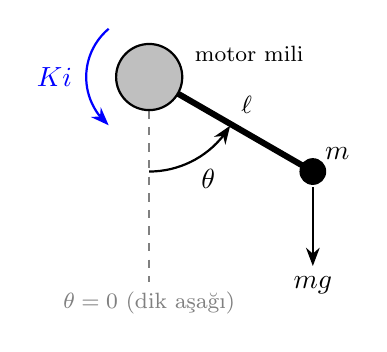
\begin{tikzpicture}[thick, >=Stealth]
  \draw[dashed, gray] (0,0) -- (0,-2.6) node[below, font=\footnotesize]{$\theta = 0$ (dik aşağı)};
  \draw[line width=2.2pt] (0,0) -- ({2.4*sin(60)},{-2.4*cos(60)})
        node[midway, above right=-1pt, font=\small]{$\ell$};
  \fill[gray!50, draw=black] (0,0) circle (0.42);
  \node[font=\footnotesize, right] at (0.45,0.3) {motor mili};
  \fill ({2.4*sin(60)},{-2.4*cos(60)}) circle (0.17)
        node[above right=1pt]{$m$};
  \draw[->] ({2.4*sin(60)},{-2.4*cos(60)-0.2}) -- ++(0,-1.0) node[below]{$mg$};
  \draw[->] (0,-1.2) arc[start angle=-90, end angle=-31, radius=1.2];
  \node at (-60:1.5) {$\theta$};
  \draw[->, blue] (130:0.8) arc[start angle=130, end angle=230, radius=0.8];
  \node[blue, left] at (180:0.85) {$K i$};
\end{tikzpicture}

\small (b) mekanik kısım (motor mili + kol)
\end{minipage}
\end{center}

Şemada tablodaki her sembolü görebiliriz: $V$, $R$, $L$, $i$ ve $K\dot\theta$ devrede; $\theta$, $\ell$, $m$, $mg$ ve $K i$ kolda. $\theta$'yı dik aşağıdan ölçüyoruz ve kol yukarı kalktıkça $\theta$ büyüyor; motor torku $K i$ da $\theta$'yı büyüten yönde.

\begin{center}
\begin{tabular}{llll}
\toprule
Sembol & Anlamı & Birim & Tür\\
\midrule
$\theta$ & kolun açısı (dik aşağıdan ölçülüyor) & rad & durum\\
$\omega = \dot\theta$ & kolun dönme hızı & rad/s & durum\\
$i$ & motor sargısındaki akım & A & durum\\
$V$ & motora uygulanan gerilim & V & giriş\\
$\theta$ & ölçülen açı (enkoder) & rad & çıkış\\
\midrule
$J_m$ & motor rotorunun dönme eylemsizliği & kg\,m$^2$ & parametre\\
$b$ & sürtünme katsayısı & N\,m\,s & parametre\\
$K$ & motor sabiti ($K = K_t = K_e$) & N\,m/A, V\,s/rad & parametre\\
$R$ & sargı direnci & $\Omega$ & parametre\\
$L$ & sargı endüktansı & H & parametre\\
$m$ & kolun ucundaki kütle & kg & parametre\\
$\ell$ & kol uzunluğu & m & parametre\\
$g$ & yerçekimi ivmesi & m/s$^2$ & parametre\\
\bottomrule
\end{tabular}
\end{center}

\subsection*{3. Hareket denklemleri ve kaynağı}

Sistemi iki parçadan oluşuyor: motorun mekanik kısmı (kolu döndüren kısım) ve elektrik kısmı (motor sargısı).

\textbf{Mekanik kısım.} Motorun ürettiği tork $K\,i$, sürtünme $b\dot\theta$ ve kolun ağırlığından gelen tork $mg\ell\sin\theta$:
\[
J\,\ddot\theta = K\,i - b\,\dot\theta - mg\ell\sin\theta, \qquad J = J_m + m\ell^2
\]
Kol dik aşağıdan ölçüldüğü için yerçekimi terimi eksi işaretli; kol yukarı kalkınca yerçekimi onu aşağı çekiyor. Toplam eylemsizlik, motorun eylemsizliğine ucunda ağırlık olan kolun eylemsizliği ($m\ell^2$) eklenerek bulunuyor.

\textbf{Elektrik kısmı.} Motor sargısı seri bir RL devresi. Kirchhoff'un gerilim yasasına göre uygulanan gerilim; dirençteki düşüm, bobindeki düşüm ve motorun dönerken ürettiği zıt gerilimin (zıt EMK, $K\dot\theta$) toplamına eşit:
\[
L\,\frac{di}{dt} = V - R\,i - K\,\dot\theta
\]

\textbf{Kaynakları.}
\begin{center}
\begin{tabular}{p{0.52\linewidth}p{0.40\linewidth}}
\toprule
Denklem parçası & Kaynak\\
\midrule
Motorun mekanik denklemi ($J\ddot\theta + b\dot\theta = K i$) & CTMS, ``DC Motor Speed: System Modeling'' [1]\\
Motorun elektrik denklemi ($L\,di/dt + R i = V - K\dot\theta$) & CTMS, aynı sayfa [1]\\
Yerçekimi terimi ($-mg\ell\sin\theta$) & Hespanha, Example 2.1 (ters sarkaç) [2]\\
Toplam eylemsizlik $J = J_m + m\ell^2$ & kolu ekleyerek bizim kurduğumuz\\
\bottomrule
\end{tabular}
\end{center}

\paragraph{Mekanik sistem formu.} Kitaptaki mekanik sistem kalıbı (2.7) şu:
\[
M(q)\,\ddot q + B(q,\dot q)\,\dot q + G(q) = F
\]
Mekanik denklemimizi bu kalıba yerleştirmek için dışarıdan gelen kuvvet dışındaki bütün terimleri sola alıyoruz; $-b\dot\theta$ ve $-mg\ell\sin\theta$ sola geçince işaretleri $+$ oluyor:
\[
J\ddot\theta + b\dot\theta + mg\ell\sin\theta = K i
\]
Kutuları eşleştirdiğimizde:

\begin{center}
\begin{tabular}{llll}
\toprule
Kalıp & Ne demek & Bizde & Anlamı\\
\midrule
$q$ & konum değişkeni & $\theta$ & kolun açısı\\
$M(q)$ & hızlandırmaya direnç & $J = J_m + m\ell^2 = 0.0105$ & eylemsizlik (sabit)\\
$B(q,\dot q)$ & hızla orantılı fren & $b = 0.1$ & sürtünme (sabit)\\
$G(q)$ & konuma bağlı kuvvet & $mg\ell\sin\theta$ & yerçekimi torku\\
$F$ & dışarıdan uygulanan & $K i$ & motor torku\\
\bottomrule
\end{tabular}
\end{center}

Kitaptaki iki eklemli kolda $M(q)$ ve $B(q,\dot q)$ açıya bağlı matrisler; bizim kolumuz tek eklemli olduğu için ikisi de sabit birer sayı. Açıya bağlı olan tek kutu $G(q) = mg\ell\sin\theta$, yani doğrusal olmayan kısmımız yine bu. Example 2.1'deki sarkaçta $F$ doğrudan giriş; bizde ise $F = K i$ akımdan geliyor ve akımı ayrı bir denklem (elektrik kısmı) belirliyor. Elektrik denklemi mekanik olmadığı için bu kalıba girmiyor; kalıba göre motor, kola tork veren bir dış kaynak.

\subsection*{4. Durum, giriş, çıkış ve model}

Durum olarak kolun açısını, dönme hızını ve motor akımını seçiyoruz: $x_1 = \theta$, $x_2 = \dot\theta$, $x_3 = i$. Giriş motor gerilimi $u = V$, çıkış ölçülen açı $y = \theta$. Kolun nereye gideceğini tahmin etmek için açıyı ve hızı bilmemiz gerekiyor; akım da motor sargısının hafızası olduğu için ayrı bir durum. 3 durum, 1 giriş, 1 çıkış: SISO bir sistem.

Soru 2'deki gibi $x_1$'in türevi $x_2$; mekanik denklemi $J$'ye, elektrik denklemini $L$'ye bölünce:
\[
\dot x_1 = x_2, \qquad
\dot x_2 = \frac{K\,x_3 - b\,x_2 - mg\ell\sin x_1}{J}, \qquad
\dot x_3 = \frac{u - R\,x_3 - K\,x_2}{L}, \qquad
y = x_1
\]

Sayıları yerine koyarken katsayılar şöyle çıkıyor:
\begin{center}
\begin{tabular}{lll}
\toprule
Katsayı & Hesap & Değer\\
\midrule
$K/J$ & $0.01 / 0.0105$ & $0.952$\\
$b/J$ & $0.1 / 0.0105$ & $9.52$\\
$mg\ell/J$ & $0.0491 / 0.0105$ & $4.67$\\
$1/L$ & $1 / 0.5$ & $2$\\
$R/L$ & $1 / 0.5$ & $2$\\
$K/L$ & $0.01 / 0.5$ & $0.02$\\
\bottomrule
\end{tabular}
\end{center}
Yani sayısal model:
\[
\dot x_1 = x_2, \qquad
\dot x_2 = 0.952\,x_3 - 9.52\,x_2 - 4.67\sin x_1, \qquad
\dot x_3 = 2\,u - 2\,x_3 - 0.02\,x_2, \qquad
y = x_1
\]
Doğrusal olmayan tek terim $\sin x_1$.

\subsection*{5. Blok diyagram}

Soru 1'deki bloklara burada bir blok daha ekleniyor: açının sinüsünü alan $\sin$ bloğu. Her durum bir integratörün çıkışı, yani 3 integratörümüz var. $\dot x_1 = x_2$ olduğu için $x_2$ integratörünün çıkışı hiçbir işlem görmeden $x_1$ integratörüne giriyor ve $y = x_1$ olduğu için $x_1$ aynı zamanda çıkış. Soldan sağa okuduğumuzda fiziksel sırayı görebiliriz: akım $\to$ hız $\to$ açı.

$\dot x_2$'nin toplama bloğuna üç terim giriyor:

\begin{center}
\small\begin{tabular}{lllll}
\toprule
Terim & Nereden & Yol & İşaret & Anlamı\\
\midrule
$0.952\,x_3$ & $x_3$ çıkışı & kazanç $0.952$ & $+$ & motor torku\\
$9.52\,x_2$ & $x_2$ çıkışı (kendi çıkışından geri) & kazanç $9.52$ & $-$ & sürtünme\\
$4.67\sin x_1$ & $x_1$ çıkışı (en sağdan geri) & önce $\sin$, sonra kazanç $4.67$ & $-$ & yerçekimi\\
\bottomrule
\end{tabular}
\end{center}

Burada sıra önemli: denklemde $4.67\sin(x_1)$ yazıyor, $\sin(4.67\,x_1)$ değil; yani önce açının sinüsünü alıp sonra $4.67$ ile çarpıyoruz.

$\dot x_3$'ün toplama bloğuna da üç terim giriyor:

\begin{center}
\small\begin{tabular}{lllll}
\toprule
Terim & Nereden & Yol & İşaret & Anlamı\\
\midrule
$2\,u$ & dışarıdan (giriş) & kazanç $1/L = 2$ & $+$ & motora verdiğimiz gerilim\\
$2\,x_3$ & $x_3$ çıkışı (kendi çıkışından geri) & kazanç $R/L = 2$ & $-$ & sargı direnci\\
$0.02\,x_2$ & $x_2$ çıkışı (ileriden geri) & kazanç $K/L = 0.02$ & $-$ & zıt EMK\\
\bottomrule
\end{tabular}
\end{center}

Son satırda hızdan akıma geri dönen bir ok var: motor hızlandıkça akım azalıyor. Elektrik ve mekanik kısım bu okla birbirine bağlanıyor.

\begin{center}
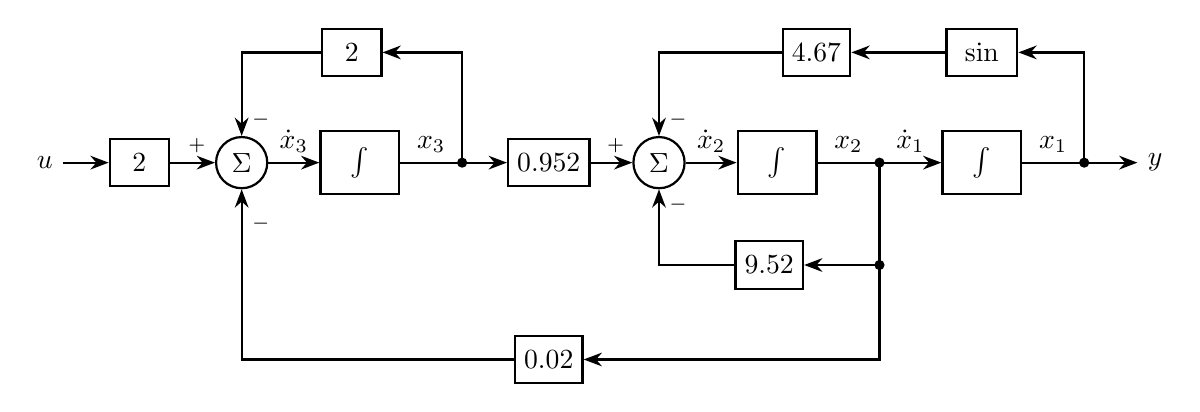
\begin{tikzpicture}[>=Stealth, thick,
  integ/.style={draw, minimum width=1.0cm, minimum height=0.8cm},
  sumb/.style={draw, circle, inner sep=0pt, minimum size=0.65cm},
  gain/.style={draw, minimum width=0.75cm, minimum height=0.6cm},
  dot/.style={circle, fill, inner sep=1.3pt},
  sgn/.style={font=\scriptsize}]
  % ileri yol
  \node (u) at (0,0) {$u$};
  \node[gain]  (gu)  at (1.2,0)  {$2$};
  \node[sumb]  (s3)  at (2.5,0)  {$\Sigma$};
  \node[integ] (i3)  at (4.0,0)  {$\int$};
  \coordinate  (c3)  at (5.3,0);
  \node[gain]  (gk)  at (6.4,0)  {$0.952$};
  \node[sumb]  (s2)  at (7.8,0)  {$\Sigma$};
  \node[integ] (i2)  at (9.3,0)  {$\int$};
  \coordinate  (c2)  at (10.6,0);
  \node[integ] (i1)  at (11.9,0) {$\int$};
  \coordinate  (c1)  at (13.2,0);
  \node (y) at (14.1,0) {$y$};
  \draw[->] (u) -- (gu);
  \draw[->] (gu) -- node[sgn, above, pos=0.6]{$+$} (s3);
  \draw[->] (s3) -- node[above]{$\dot x_3$} (i3);
  \draw (i3) -- node[above]{$x_3$} (c3);
  \draw[->] (c3) -- (gk);
  \draw[->] (gk) -- node[sgn, above, pos=0.6]{$+$} (s2);
  \draw[->] (s2) -- node[above]{$\dot x_2$} (i2);
  \draw (i2) -- node[above]{$x_2$} (c2);
  \draw[->] (c2) -- node[above]{$\dot x_1$} (i1);
  \draw (i1) -- node[above]{$x_1$} (c1);
  \draw[->] (c1) -- (y);
  \node[dot] at (c3) {}; \node[dot] at (c2) {}; \node[dot] at (c1) {};
  % x3 -> sargi direnci (ust)
  \node[gain] (gr) at (3.9,1.4) {$2$};
  \draw[->] (c3) |- (gr);
  \draw[->] (gr) -| node[sgn, pos=0.9, right]{$-$} (s3);
  % x1 -> sin -> yercekimi (ust)
  \node[draw, minimum width=0.9cm, minimum height=0.6cm] (sn) at (11.9,1.4) {$\sin$};
  \node[gain] (gg) at (9.8,1.4) {$4.67$};
  \draw[->] (c1) |- (sn);
  \draw[->] (sn) -- (gg);
  \draw[->] (gg) -| node[sgn, pos=0.9, right]{$-$} (s2);
  % x2 -> surtunme (alt)
  \coordinate (d2) at (10.6,-1.3);
  \node[gain] (gb) at (9.2,-1.3) {$9.52$};
  \draw (c2) -- (d2);
  \node[dot] at (d2) {};
  \draw[->] (d2) -- (gb);
  \draw[->] (gb) -| node[sgn, pos=0.9, right]{$-$} (s2);
  % x2 -> zit EMK (en alt)
  \node[gain] (ge) at (6.4,-2.5) {$0.02$};
  \draw[->] (d2) |- (ge);
  \draw[->] (ge) -| node[sgn, pos=0.9, right]{$-$} (s3);
\end{tikzpicture}
\end{center}

Kontrol ettiğimizde 3 integratör (3 durum), 6 kazanç (madde 4'teki 6 katsayı), 2 toplama bloğu ve 1 $\sin$ bloğu görüyoruz; her denklemdeki her terimin bir oku var. Diyagramdaki doğrusal olmayan tek blok $\sin$. Madde 7'de 90° etrafında doğrusallaştırdığımızda bu blok $\cos 90^\circ = 0$ kazancına dönüşüyor ve yerçekimi yolu kayboluyor; madde 8'deki $0$ özdeğeri de buradan geliyor.

\subsection*{6. Parametre değerleri ve kaynakları}

\begin{center}
\begin{tabular}{llll}
\toprule
Parametre & Değer & Kaynak & Not\\
\midrule
$J_m$ & $0.01$ kg\,m$^2$ & CTMS [1] & \\
$b$ & $0.1$ N\,m\,s & CTMS [1] & \\
$K$ & $0.01$ N\,m/A & CTMS [1] & $K_t = K_e$\\
$R$ & $1\ \Omega$ & CTMS [1] & \\
$L$ & $0.5$ H & CTMS [1] & \\
$m$ & $0.05$ kg & tasarım hesabı & aşağıda\\
$\ell$ & $0.1$ m & tasarım hesabı & aşağıda\\
$g$ & $9.81$ m/s$^2$ & & \\
$J$ & $0.0105$ kg\,m$^2$ & $J_m + m\ell^2$ & $0.01 + 0.05\cdot 0.1^2$\\
\bottomrule
\end{tabular}
\end{center}

\textbf{Kol ölçülerinin tasarım hesabı.} Motor sabiti küçük ($K = 0.01$ N\,m/A), yani 1 A akımla yalnızca 0.01 N\,m tork üretiyor. Kol ağır olursa motor onu kaldıramaz. Bu yüzden hafif bir kol seçtik ve motorun onu en zor durumda, yani yatayda ($\sin 90^\circ = 1$) tutabildiğini kontrol ettik:
\begin{itemize}[leftmargin=*]
  \item Yerçekiminin torku: $mg\ell = 0.05 \times 9.81 \times 0.1 \approx 0.049$ N\,m
  \item Gereken akım: $0.049 / 0.01 \approx 4.9$ A
  \item Gereken gerilim (kol dururken): $R\,i = 1 \times 4.9 \approx 4.9$ V
\end{itemize}
12 V'luk bir besleme bunu rahatça karşılıyor, yani motor kolu her açıda tutabiliyor.

\subsection*{7. Denge noktaları}

Kolu $\theta_0$ açısında tutmak istiyoruz. Dengede bütün değişim hızları sıfır olmalı:
\begin{itemize}[leftmargin=*]
  \item $\dot x_1 = 0 \;\Rightarrow\; x_2 = 0$. Kol dönmüyor.
  \item $\dot x_2 = 0$: $x_2 = 0$ yazınca $0.952\,x_3 = 4.67\sin\theta_0$, yani $x_3 = (4.67/0.952)\sin\theta_0 \approx 4.9\sin\theta_0$. Bu, motorun yerçekimini dengelemesi için gereken akım.
  \item $\dot x_3 = 0$: $x_2 = 0$ yazınca $2u = 2x_3$, iki tarafı 2'ye bölünce $u = x_3$.
\end{itemize}
Yani denge noktası:
\[
x^{eq} = \big(\theta_0,\ 0,\ 4.9\sin\theta_0\big), \qquad u^{eq} = 4.9\sin\theta_0\ \text{V}
\]

\begin{center}
\begin{tabular}{llll}
\toprule
Açı $\theta_0$ & Akım $x_3$ & Gerilim $u^{eq}$ & Anlamı\\
\midrule
$0$ (asılı) & 0 A & 0 V & motorun bir şey yapmasına gerek yok\\
$45^\circ$ & 3.5 A & 3.5 V & \\
$90^\circ$ (yatay) & 4.9 A & 4.9 V & en zor durum, motor kolun bütün ağırlığını taşıyor\\
\bottomrule
\end{tabular}
\end{center}

Kol yatayken bulduğumuz 4.9 A ve 4.9 V, kol ölçülerini seçerken yaptığımız tasarım hesabıyla aynı; model ve hesap birbirini doğruluyor. Soru 2(c)'deki sarkaçta motorun gücü bazı açılara yetmiyordu; burada kolu hafif seçtiğimiz için her açıda denge kurulabiliyor.

\textbf{Projede kullanacağımız denge noktası:} $\theta_0 = 90^\circ$ (kol yatay). Hem en zor durum hem de kontrol açısından en ilginç olanı.

\subsection*{8. Açık çevrim simülasyonu}

Motora sabit denge gerilimini veriyoruz ve kolu 90°'nin biraz altından, tam üstünden ve biraz üstünden bırakıyoruz. Gerilimi parametrelerden yuvarlamadan hesapladığımızda $u = R\,mg\ell/K = 4.905$~V çıkıyor (madde 7'deki 4.9 bunun yuvarlanmış hali). Akım başlangıçta dengedeki değerinde ($x_3(0) = 4.905$~A), hız sıfır. Denklemleri MATLAB'da \texttt{ode45} ile 60~s boyunca çözüyoruz (\texttt{kt1.m}).

\begin{center}
\begin{tabular}{llll}
\toprule
Giriş & Başlangıç & Süre & Çıkış\\
\midrule
$u = 4.905$~V (sabit) & $\theta(0) = 80^\circ,\ 90^\circ,\ 100^\circ$; $\omega(0)=0$; $i(0) = 4.905$~A & 60~s & $y = \theta(t)$\\
\bottomrule
\end{tabular}
\end{center}

\begin{figure}[H]
\centering
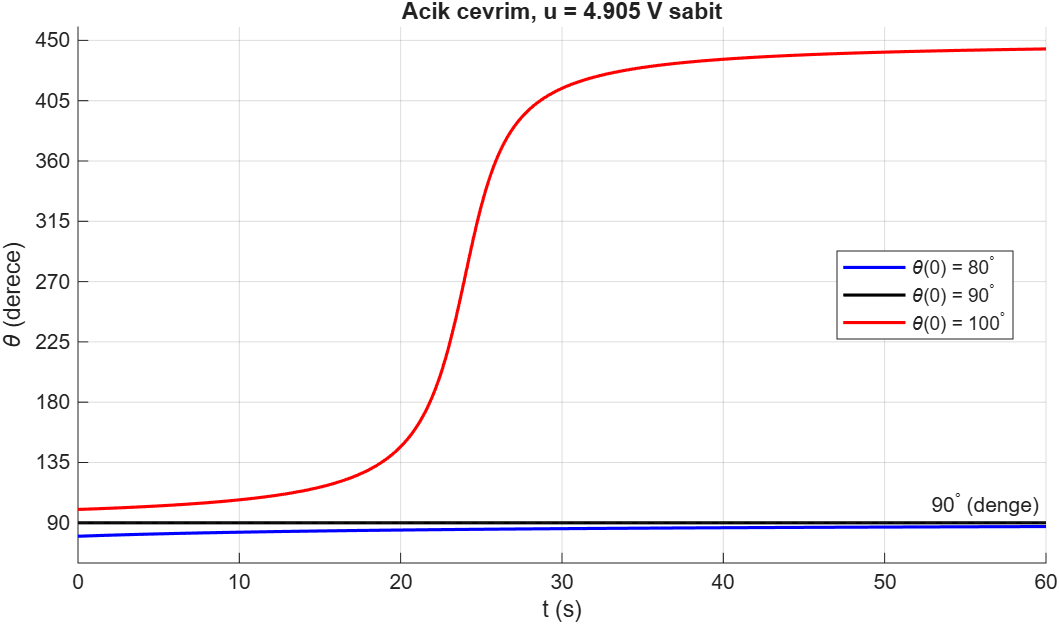
\includegraphics[width=0.8\linewidth]{../sekiller/kt1_acik_cevrim.png}
\caption{Sabit $u = 4.905$~V ile üç başlangıç açısı için $\theta(t)$.}
\end{figure}

\begin{center}
\begin{tabular}{lll}
\toprule
$\theta(0)$ & $\theta(60\text{ s})$ & Ne oldu?\\
\midrule
$80^\circ$ & $87.2^\circ$ & 90°'ye doğru çok yavaş yaklaşıyor\\
$90^\circ$ & $90.0^\circ$ & hiç kıpırdamıyor\\
$100^\circ$ & $443.6^\circ$ & uzaklaşıyor, tam bir tur dönüp tekrar 90°'ye ($450^\circ$) geliyor\\
\bottomrule
\end{tabular}
\end{center}

Bunun nedenini torklara bakarak görebiliriz. Motorun torku sabit: $K i = 0.01 \times 4.905 = 0.049$~N\,m. Yerçekiminin torku $mg\ell\sin\theta$ ve en büyük değeri olan 0.049'a tam 90°'de ulaşıyor. Yani 90°'de iki tork eşit, kol duruyor. 80°'de ve 100°'de ise $\sin\theta < 1$ olduğu için yerçekimi daha zayıf ve motor kazanıyor; motor kolu her iki durumda da yukarı itiyor. 80°'de yukarısı 90°'ye doğru olduğu için kol dengeye yaklaşıyor. 100°'de ise yukarısı 90°'den uzağa doğru, kol tepeden geçiyor, düşerken yerçekimi de yardım ediyor ve tam bir tur atıyor.

Aynı sonucu özdeğerlerden de görebiliriz. 90°'de doğrusallaştırdığımızda özdeğerler $0$, $-9.52$ ve $-2.00$ çıkıyor. $-9.52$ ve $-2.00$ sürtünmeden ve motorun elektrik kısmından gelen hızlı sönümler. $0$ ise $\cos 90^\circ = 0$ olmasından geliyor: bu noktada yerçekiminin eğimi sıfır, kolu geri itecek bir etki yok. Soru 4'teki lamba/kalem durumlarının ikisi de değil; masanın kenarında duran bir bilye gibi, bir yana itersek geri geliyor, öbür yana itersek düşüyor. 80° eğrisinin bu kadar yavaş yaklaşması da bu sıfır özdeğerden.

Aşağıdaki film şeridi 100° durumunun animasyonundan seçtiğimiz anları gösteriyor (kesikli çizgi 90°, gri kare motor):

\begin{figure}[H]
\centering
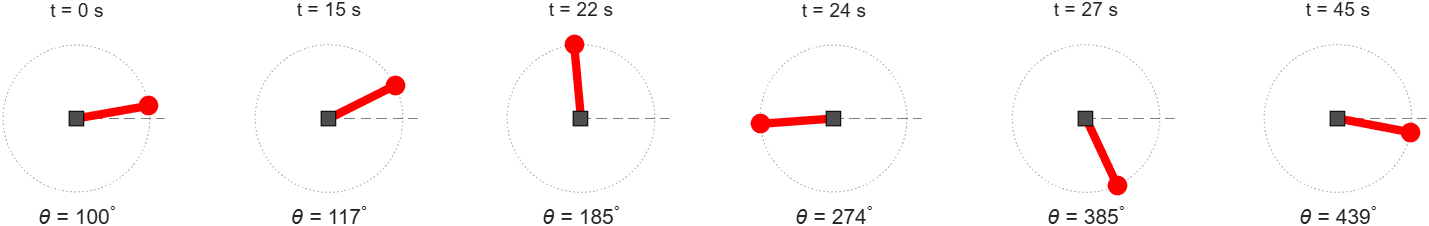
\includegraphics[width=\linewidth]{../sekiller/kt1_filmseridi.png}
\caption{$\theta(0)=100^\circ$: kol tepeden geçip ($t=22$~s) tam tur atıyor ve 90°'ye geri geliyor.}
\end{figure}

Üç durumun animasyonunun tamamını \texttt{kt1\_animasyon.m} ile ürettik; GIF dosyası: \url{sekiller/kt1_animasyon.gif}.

Yani sabit gerilim verip bırakmak kolu 90°'de güvenle tutmaya yetmiyor; küçük bir sapma kolu tam tura gönderebiliyor. Projenin devamında geri besleme eklememizin nedeni bu.

\subsection*{Kaynaklar}
\begin{enumerate}[label={[\arabic*]}, leftmargin=*]
  \item B. Messner, D. Tilbury, R. Hill, \emph{Control Tutorials for MATLAB and Simulink}, ``DC Motor Speed: System Modeling,'' University of Michigan. \url{https://ctms.engin.umich.edu/CTMS/index.php?example=MotorSpeed&section=SystemModeling} (erişim: 13 Ekim 2026)
  \item J. P. Hespanha, \emph{Linear Systems Theory}, Princeton University Press, 2009, Example 2.1.
\end{enumerate}

%======================================================================

\end{document}
